%% --------------------------------------------------------------
%%
%% I N T R O D U C T I O N
%%
%% --------------------------------------------------------------
\section{Introduction}


\begin{frame}{}  %% ---------- Intro/motivation 
    \begin{tikzpicture}[overlay,remember picture]
        
        \uncover<1->{ % <-> |
            \node (t1) [anchor=center,scale=1,opacity=1] at ([shift={(-3.0cm,-0.28cm)}]current page.center){
                \parbox{0.7\textwidth}{
                    \begin{itemize}
                        \item Short gamma-ray bursts (sGRB) and kilonovae (kN) -- electromagnetic counterparts of (at least some) binary neutron star mergers (BNS). 
                        \item \textbf{Afterglow} -- non-thermal emission from electrons in (external) shocks created by ejecta moving through ISM. 
                        \item GRBs, kNe and their afterglows $\propto$ properties of ejecta.
                        \item Ejecta properties $\propto$ (i) binary properties, \\(ii) \textbf{NS equation of state}.
                    \end{itemize}
%                    Short gamma-ray burst (likely) projenitors are compact object mergers
%                    \textbf{Messengers:}
%                    \begin{itemize}
%                        \item Gravitational Waves
%                        \item Neutrino emission
%                        \item Gamma-ray burst (GRB) 
%                        \item Kilonova (kN): thermal radiation from decay of newly produced heavy nuclei
%                        \item \textbf{GRB afterglow}: non-thermal emission produced by GRB ejecta sweeping-up ISM
%                        \item \textbf{Kilonova afterglow}: non-thermal emission produced by kN ejecta sweeping up ISM
%                    \end{itemize}
%                    Numerical relativity simulations $\rightleftarrows$ EM transient models
            }};
            
        }
        
%        \uncover<1->{ % <-> |
%            \node (t1) [anchor=center,scale=1,opacity=1] at ([shift={(-3.0cm,-0.28cm)}]current page.center){
%                \parbox{0.7\textwidth}{
%                    Binary Neutron Star (BNS) and Neutron Star Black Hole (NSBH) mergers expose 
%                    properties of matter at densities many times the nuclear saturation density. \\
%                    \textbf{Messengers:}
%                    \begin{itemize}
%                        \item Gravitational Waves
%                        \item Neutrino emission
%                        \item Gamma-ray burst (GRB) 
%                        \item Kilonova (kN): thermal radiation from decay of newly produced heavy nuclei
%                        \item \textbf{GRB afterglow}: non-thermal emission produced by GRB ejecta sweeping-up ISM
%                        \item \textbf{Kilonova afterglow}: non-thermal emission produced by kN ejecta sweeping up ISM
%                    \end{itemize}
%                    Numerical relativity simulations $\rightleftarrows$ EM transient models
%            }};
%            
%        }
%            \uncover<1->{ % <-> |
%        \node (t1) [anchor=center,scale=1,opacity=1] at ([shift={(-3.5cm,-0.5cm)}]current page.center){
%            \parbox{0.6\textwidth}{
%                \begin{itemize}
%                    \item One of the ways to understand the properties of matter at supernuclear densities 
%                    is to study EM signatures of BNS, NSBH mergers and CCSNe. 
%                    %
%                    \item Non-thermal EM signatures: GRBs, kN afterglows, ... 
%                    %
%                    \item Origin: interaction between transrelativistic ejecta and ISM. 
%                    %
%                    \item Thus study of GRBs, kN probe the ejecta properties and by extension, the 
%                    properties of the postmerger/post-SNe remnant. 
%                    \item NR simulations + observations show 
%                \end{itemize}
%        }};
%        
%    }
        \uncover<1-1>{ % <-> |
            \node (img1) [anchor=center,scale=1,opacity=1] at ([shift={(5.6cm,-0.8cm)}]current page.center){
                \parbox{0.5\textwidth}{
                    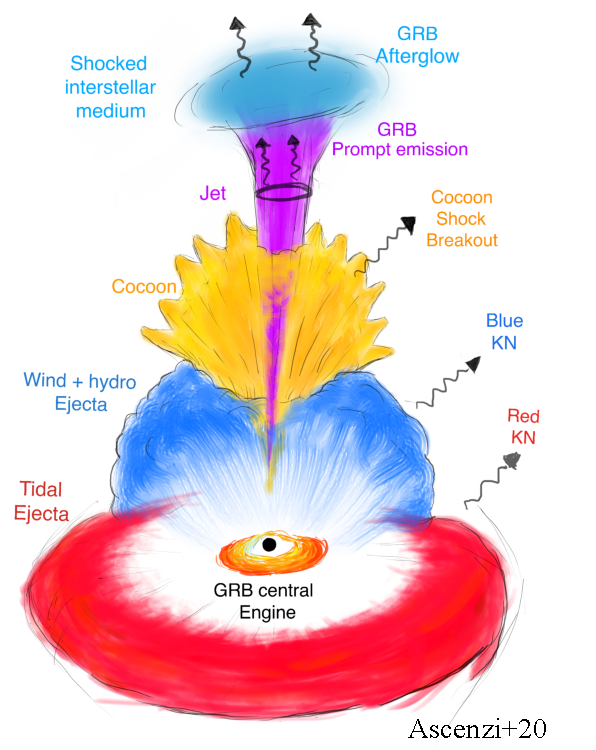
\includegraphics[height=7.0cm]{../figs/Ascenzi20_EjectaEMPicture.pdf}
                    
                    %\small{\textbf{Artist depiction of ejecta$^\text{\citep{Ascenzi:2020xqi}}$}}
            }};
        }
    \end{tikzpicture}
\end{frame}

% =============================================================================================

\section{Observations}
\begin{frame}{}  %% ---------- Intro/motivation 
    \begin{tikzpicture}[overlay,remember picture]
        \uncover<1->{ % <-> |
            \node (t1) [anchor=center,scale=1,opacity=1] at ([shift={(-4.cm,2.0cm)}]current page.center){
                \parbox{0.6\textwidth}{
                    \begin{itemize}
                        \item GRB afterglow $+$ kilonova \textcolor{darkgreen}{\cmark}
                        \item GRB and kilonova ejecta have structure \\
                        \item Off-axis observations \\
                        \item Multi-messenger sources 
                    \end{itemize}
            }};
        }

        \uncover<1-1>{ % <-> |
            \node (img1) [anchor=center,scale=1,opacity=1] at ([shift={(1.2cm,-2.1cm)}]current page.center){
                \parbox{0.5\textwidth}{
                    \GRB{} \\
                    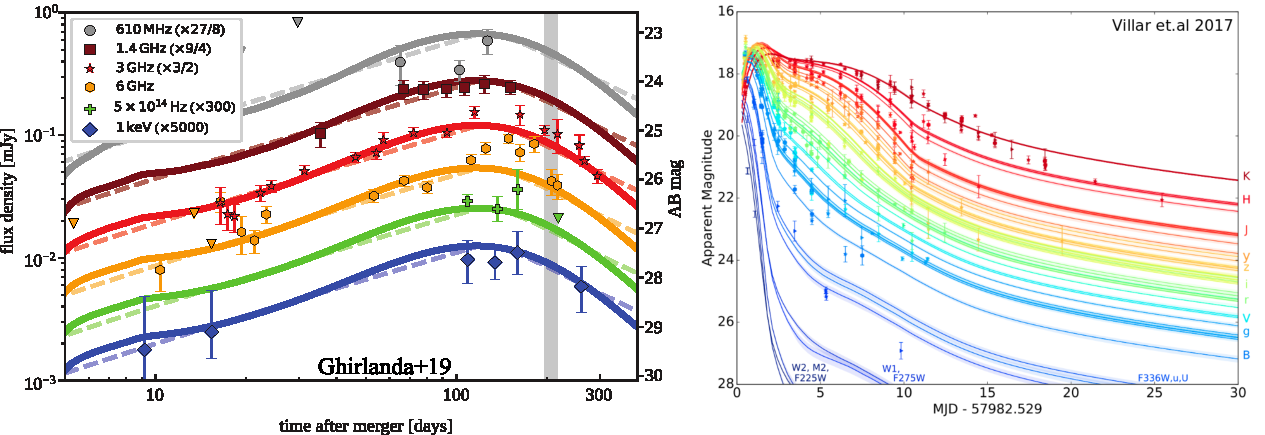
\includegraphics[height=3.5cm]{../figs/Chirlanda_Villar_170817.pdf}
            }};
        }
        \uncover<1-1>{ % <-> |
        \node (img1) [anchor=center,scale=1,opacity=1] at ([shift={(3.2cm,1.6cm)}]current page.center){
            \parbox{0.5\textwidth}{
                GRB211211A \\
                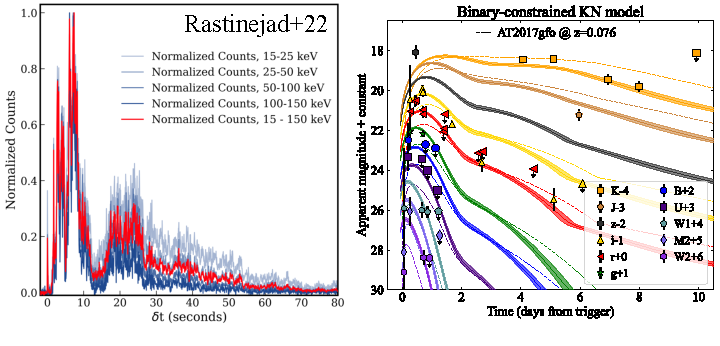
\includegraphics[height=3.7cm]{../figs/Rastinejad22_GRB211211_2.pdf}
        }};
        }
%        \uncover<1-1>{ % <-> |
%            \node (img1) [anchor=center,scale=1,opacity=1] at ([shift={(1.5cm,-1.8cm)}]current page.center){
%                \parbox{0.5\textwidth}{
%                    \GRB{} \\ 
%                    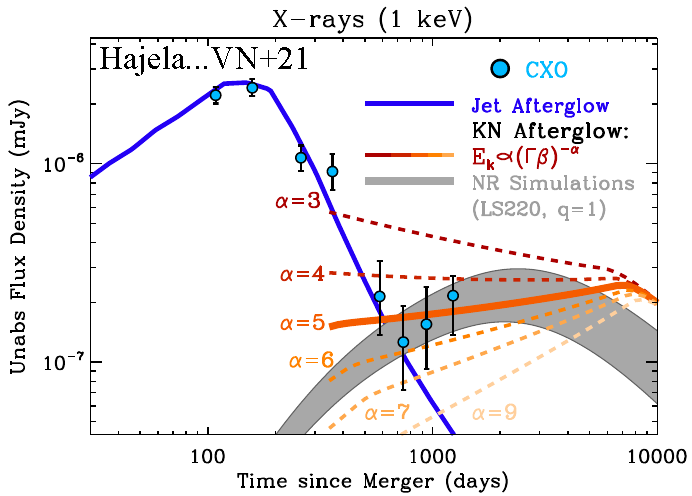
\includegraphics[height=4.0cm]{../figs/Hajela21_ChangeGW170817-2.pdf}
%            }};
%        }
        \uncover<1-1>{ % <-> |
            \node (img1) [anchor=center,scale=1,opacity=1] at ([shift={(-4.0cm,-1.85cm)}]current page.center){
                \parbox{0.5\textwidth}{
                    GRB160821B \\
                    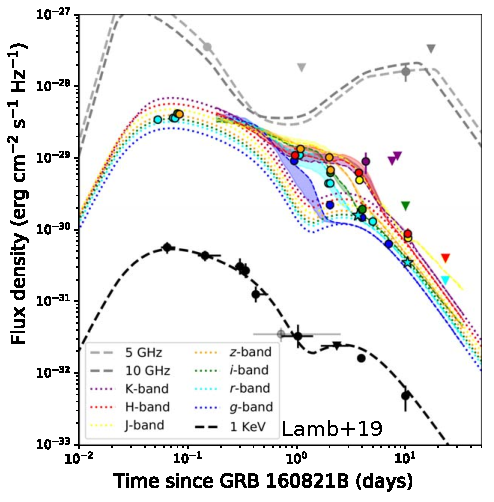
\includegraphics[height=4.02cm]{../figs/Lamb19_GRB160821B.pdf}
            }};
        }
    \end{tikzpicture}
\end{frame}

\section{Kilonova afterglow}
\begin{frame}{}  %% ---------- Intro/motivation 
    \begin{tikzpicture}[overlay,remember picture]
        \uncover<1->{ % <-> |
            \node (t1) [anchor=center,scale=1,opacity=1] at ([shift={(-3.2cm,1.7cm)}]current page.center){
                \parbox{0.65\textwidth}{
                    \textbf{Kilonova afterglow}:\\ 
                    Peaks in radio bands on timescale of years \\
                    \hspace*{5mm}\textcolor{gray}{\footnotesize{(Nakar, E., Piran, T., 2011, Nature 478)}} \\
                    Velocity and angular ejecta distribution are important \\ 
                    \hspace*{5mm}\textcolor{gray}{\footnotesize{(Piran, T., Nakar, E., Rosswog, S., 2013, MNRAS 430 3)}} \\
                    Expected but so far not observed\textcolor{red}{*} \\
                    \hspace*{5mm}\textcolor{gray}{\footnotesize{(Hajela, A., ... VN et.~al., 2021, ApJL 927 1, L17)}}\\ 
                    \textcolor{red}{*}\textit{GRB170817A late time light curve change}
%                    GRB afterglow $+$ kilonova \textcolor{darkgreen}{\cmark} \\
%                    GRB afterglow $+$ kilonova afterlow -- not yet \textcolor{red}{\xmark}
%                    \begin{itemize}
%                        \item shallow rising light curve: structured, off-axis
%                        \item late time flattening: lateral spreading, emergence of another component 
%                        % (spectral evolution)
%                        %                        \textit{harder radio-to-X-ray spectrum} (lower $p$)
%                        %                        \item Radio obs. $\rightarrow$ optically thin spectrum
%                        %                        \item Lower $p=2$ \textit{is expected} in non-relativistic shocks (but with lower $\varepsilon_e$ as well)
%                    \end{itemize}
            }};
        }
%        \uncover<1->{ % <-> |
%            \node (t1) [anchor=center,scale=1,opacity=1] at ([shift={(-5.9cm,-2.0cm)}]current page.center){
%                \parbox{0.3\textwidth}{
%                    %\textbf{ Afterglow characteristics }
%                    \begin{equation*}
%                        \begin{aligned}
%                            F_{\nu,p} & \propto E n^{(p+1)/4}  
%                            \textcolor{red}{ \beta^{(5p-7)/2} }   \\
%                            & \times \varepsilon_e^{p-1}\varepsilon_B^{(p+1)/4} \\
%                            & \times D_L^{-2}\nu^{(-p-1)/2} \\
%                            t_{p} & \propto E^{1/3} n^{-1/3} 
%                            \textcolor{red}{ \beta^{-5/3} }
%                        \end{aligned}
%                    \end{equation*}
%            }};
%        }
        %        \uncover<1->{ % <-> |
            %        \node (t1) [anchor=center,scale=1,opacity=1] at ([shift={(-5.5cm,0.7cm)}]current page.center){
                %            \parbox{0.4\textwidth}{
                    %                No unambigous detection of GRB + kN afterglows. Possible candidates: GRB160821B and \GRB{}.
                    %                GRB170817 from [Hajela et al 2021]:
                    %                \begin{itemize}
                        %                    %                        \item late-time cahnge in afterglow (not a jet)
                        %                    \item Statistical fit indicates
                        %                    \textit{harder radio-to-X-ray spectrum} (lower $p$)
                        %                    \item Radio obs. $\rightarrow$ optically thin spectrum
                        %                    \item Lower $p=2$ \textit{is expected} in non-relativistic shocks (but with lower $\varepsilon_e$ as well)
                        %                \end{itemize}
                    %                
                    %        }};
            %        }
        \uncover<1-1>{ % <-> |
            \node (img1) [anchor=center,scale=1,opacity=1] at ([shift={(-0.5cm,-2.35cm)}]current page.center){
                \parbox{0.5\textwidth}{
                    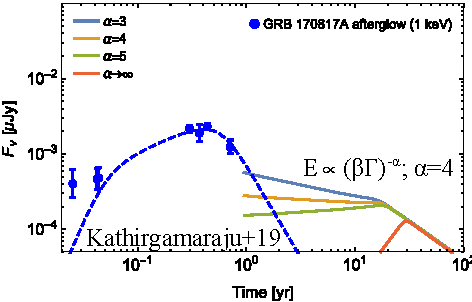
\includegraphics[height=3.8cm]{../figs/Kathirgamaraju19_kN_afg_to_GRB170817A_xray.pdf}
            }};
        }
%        \uncover<1-1>{ % <-> |
%            \node (img1) [anchor=center,scale=1,opacity=1] at ([shift={(-4.2cm,-1.8cm)}]current page.center){
%                \parbox{0.5\textwidth}{
%                    \GRB{} \\
%                    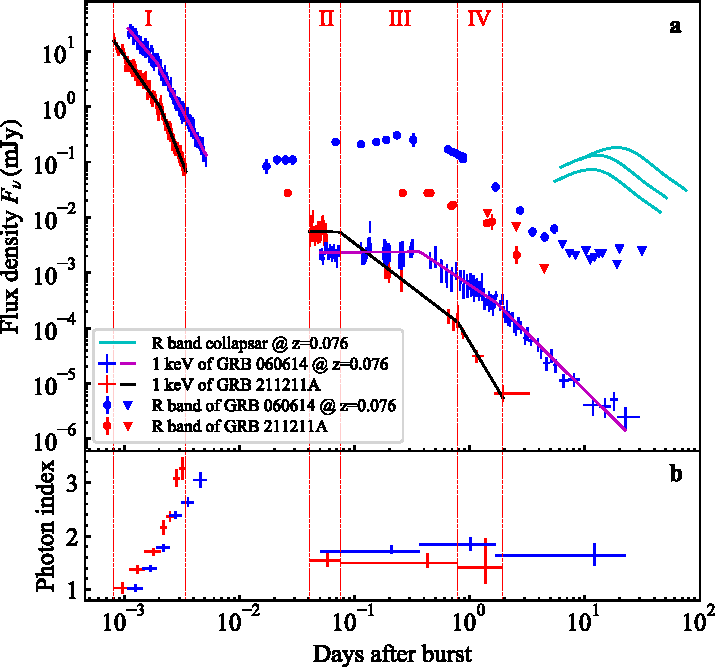
\includegraphics[height=4.0cm]{../figs/Yang22_GRB211211A.pdf}
%            }};
%        }
        \uncover<1-1>{ % <-> |
            \node (img1) [anchor=center,scale=1,opacity=1] at ([shift={(5.6cm,1.8cm)}]current page.center){
                \parbox{0.5\textwidth}{
                    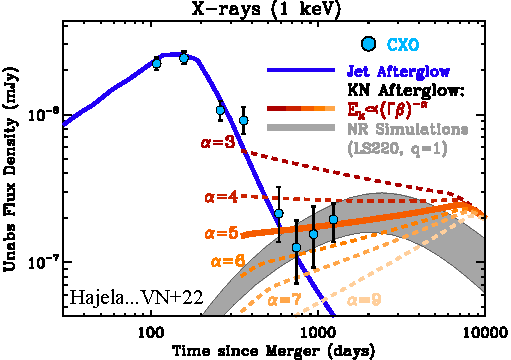
\includegraphics[height=4.0cm]{../figs/Hajela21_ChangeGW170817_xray.pdf}
            }};
        }
        \uncover<1-1>{ % <-> |
        \node (img1) [anchor=center,scale=1,opacity=1] at ([shift={(5.6cm,-2.2cm)}]current page.center){
            \parbox{0.5\textwidth}{
                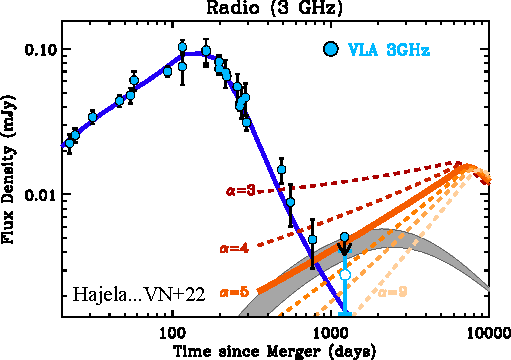
\includegraphics[height=4.0cm]{../figs/Hajela21_ChangeGW170817_radio.pdf}
        }};
        }
%        \uncover<1-1>{ % <-> |
%            \node (img1) [anchor=center,scale=1,opacity=1] at ([shift={(7.0cm,-1.8cm)}]current page.center){
%                \parbox{0.5\textwidth}{
%                    GRB160821B \\
%                    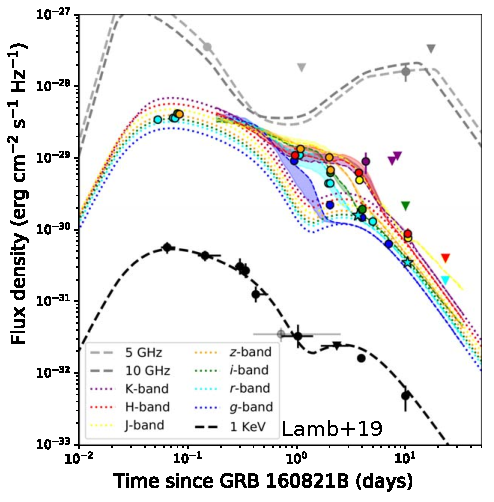
\includegraphics[height=4.02cm]{../figs/Lamb19_GRB160821B.pdf}
%            }};
%        }
    \end{tikzpicture}
\end{frame}

% =============================================================================================

%\section{Kilonova afterglow}
\begin{frame}{}  %% ---------- Intro/motivation 
    \begin{tikzpicture}[overlay,remember picture]
        \uncover<1->{ % <-> |
            \node (t1) [anchor=center,scale=1,opacity=1] at ([shift={(-3.7cm,2.0cm)}]current page.center){
                \parbox{0.60\textwidth}{
                    \textbf{ Numerical relativity simulations show}:
                    \begin{itemize}
                        \item presence of the dynamial ejecta \textit{fast tail},
%                        \item ejecta properties depend in the binary parameters
                        \item complex velocity- \& lateral- structure. 
                    \end{itemize}
                    \begin{equation*}
                        \tilde{\Lambda} := \frac{16}{13}\frac{(M_A + 12M_B)M_A^4}{M^5}+(A\leftrightarrow B).
                    \end{equation*}
                    $ q=M_A / M_B$; $ \{ M_{\rm ej}, \Gamma_{\rm ej} \} = f(q,\tilde{\Lambda}) = f(\text{EOS})$
%                    $\downarrow\tilde{\Lambda}$ for softer EOS, $\uparrow M$, $\uparrow q=M_A/M_B$ \\
%                    \textbf{Key Observables}: 
%                    \begin{itemize}
%                        \item $F_{\nu,p}\propto E n^{(p+1)/4}\beta^{(5p-7)/2}\varepsilon_e^{p-1}\varepsilon_B^{(p+1)/4}D_L^{-2}\nu^{(-p-1)/2}$
%                        \item $t_{p}\propto E^{1/3} n^{-1/3} \beta^{-5/3}$
%                        %
%                        \item Timescale of years.
%                        %
%                        \item Trace the properties of the fastest ejecta
%                        %
%                    \end{itemize}
            }};
        }
        \uncover<1-2>{ % <-> |
            \node (img1) [anchor=center,scale=1,opacity=1] at ([shift={(3.4cm,3.40cm)}]current page.center){
                \parbox{0.35\textwidth}{
                    \textcolor{gray}{\footnotesize{NV, Radice D., Bernuzzi S., et al., 2021, MNRAS, 506, 5908}}
            }};
        }
        \uncover<1-1>{ % <-> |
            \node (img1) [anchor=center,scale=1,opacity=1] at ([shift={(4.1cm,-0.7cm)}]current page.center){
                \parbox{0.5\textwidth}{
                    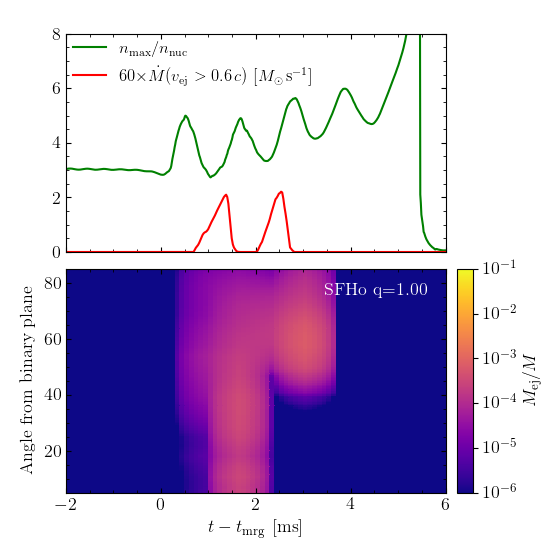
\includegraphics[height=7.4cm]{../figs/SFHo_q100_LK_SR.png}
                    %\small{\textbf{Artist depiction of ejecta$^\text{\citep{Ascenzi:2020xqi}}$}}
            }};
        }
        \uncover<1-1>{ % <-> |
        \node (img1) [anchor=center,scale=1,opacity=1] at ([shift={(-3.2cm,-1.85cm)}]current page.center){
            \parbox{0.5\textwidth}{
                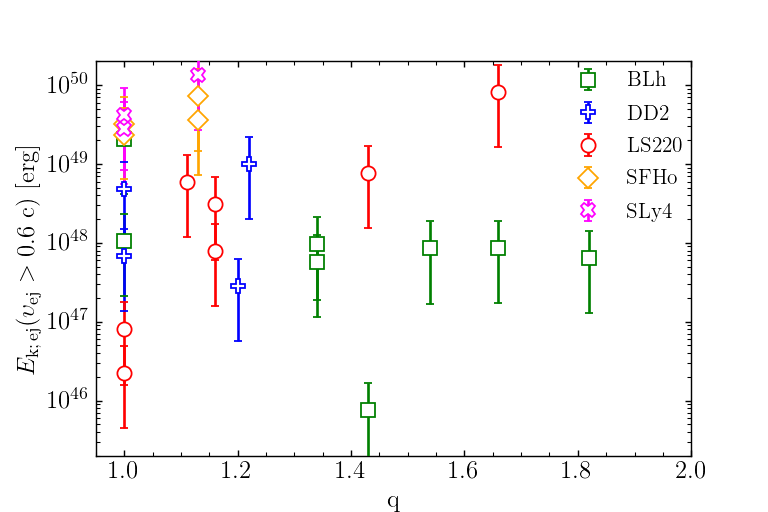
\includegraphics[height=4.4cm]{../figs/scatter_ekej_vej06.png}
                %\small{\textbf{Artist depiction of ejecta$^\text{\citep{Ascenzi:2020xqi}}$}}
        }};
        }
        \uncover<2-2>{ % <-> |
            \node (img1) [anchor=center,scale=1,opacity=1] at ([shift={(-3.2cm,-1.85cm)}]current page.center){
                \parbox{0.5\textwidth}{
                    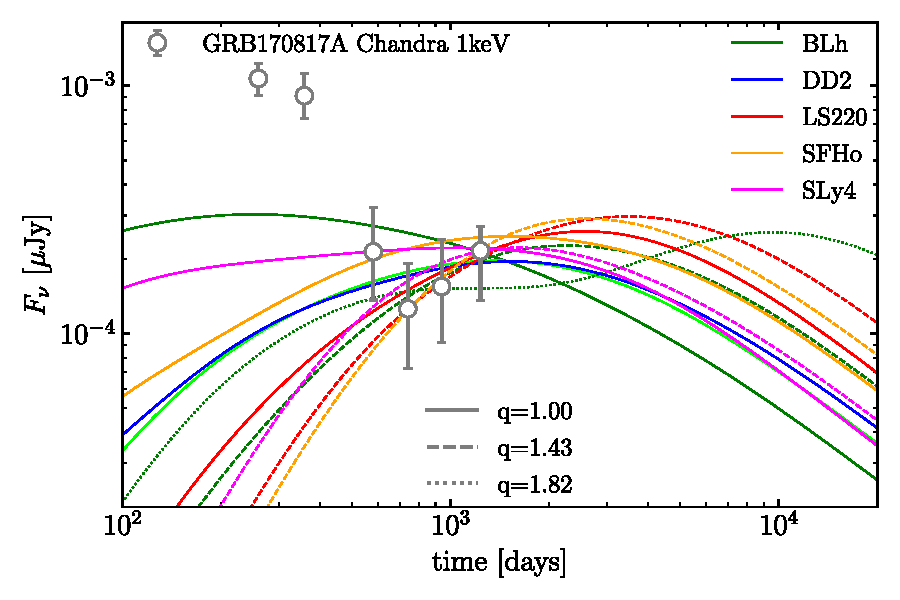
\includegraphics[height=4.4cm]{../figs/best_xray_obs_representative_all_eos.pdf}
                    %\small{\textbf{Artist depiction of ejecta$^\text{\citep{Ascenzi:2020xqi}}$}}
            }};
        }
        \uncover<2->{ % <-> |
            \node (t1) [anchor=center,scale=1,opacity=1] at ([shift={(4.6cm,1.7cm)}]current page.center){
                \parbox{0.60\textwidth}{
                    \textbf{NR-informed light curves show}:
                    \begin{itemize}
                        \item consistency with observations; %$(t_p, F_{\nu=1\text{keV} p})$ 
                        \item very energetic ejecta disfavoured;
                        \item $\rightarrow$ low $\tilde{\Lambda}$ and $q=1$ disfavoured.
                    \end{itemize}
            }};
        }
        \uncover<2-2>{ % <-> |
            \node (img1) [anchor=center,scale=1,opacity=1] at ([shift={(5.0cm,-1.9cm)}]current page.center){
                \parbox{0.60\textwidth}{
                    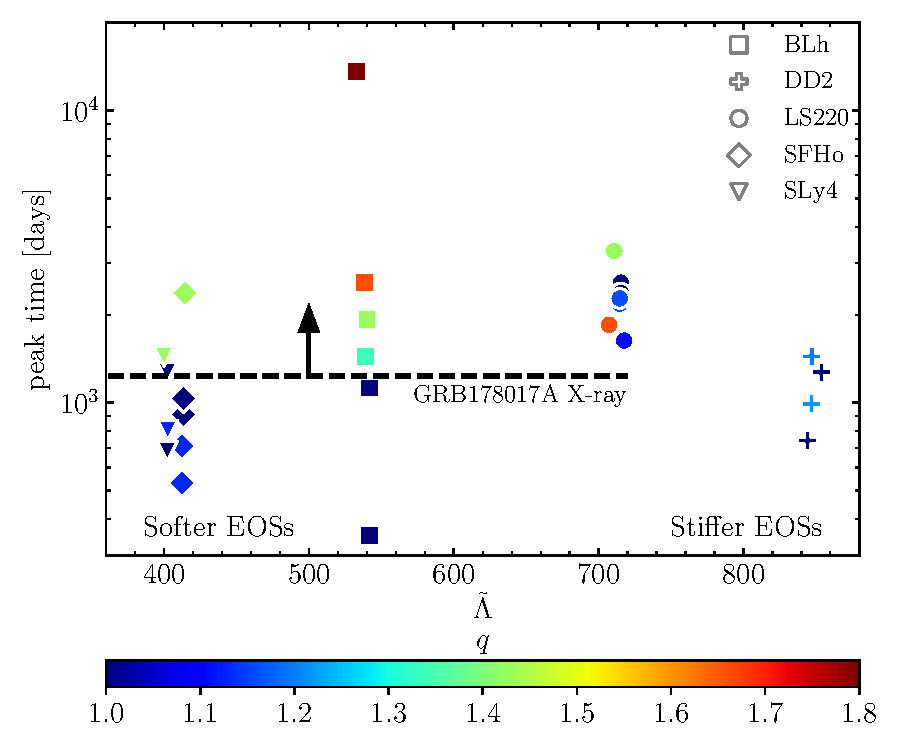
\includegraphics[height=4.9cm]{../figs/scatter_lightcurve_tpeak_vs_lambda.pdf}
                    %\includesvg[height=7.2cm]{figures/structure2}
            }};
        }
    \end{tikzpicture}
\end{frame}

% =============================================================================================

\section{Model}
\begin{frame}{}  %% ---------- Intro/motivation 
    \begin{tikzpicture}[overlay,remember picture]
        \uncover<1->{ % <-> |
            \node (t1) [anchor=center,scale=1,opacity=1] at ([shift={(-4.0cm,-0.1cm)}]current page.center){
                \parbox{0.57\textwidth}{
                    \textbf{GRB and kN ejecta interact twice}: 
                    \begin{itemize}
                        \item \normalsize{GRB ejecta breaks out of kN ejecta} \\ \textcolor{gray}{\footnotesize{(Nativi et al., 2021, MNRAS, 500, 1772)},}
                        \item  \normalsize{kN ejecta polws through GRB ejecta} \textcolor{gray}{(\footnotesize{Margalit B., Piran T., 2020, MNRAS, 495, 4981)}.}
                    \end{itemize}
                    \vspace{5mm}
                    \textbf{Unknowns}:
                    \begin{itemize}
                        \item will NR-informed kilonova ejecta "catch up" with observations-informed GRB one and when?
                        \item how the GRB ejecta evacuating ISM affects kN ejecta dynamics \& emission?
                    \end{itemize}
                }};
            
        }
        \uncover<1-1>{ % <-> |
            \node (img1) [anchor=center,scale=1,opacity=1] at ([shift={(4.5cm,-0.3cm)}]current page.center){
                \parbox{0.6\textwidth}{
                    \includegraphics[height=7.8cm]{../figs/structure2.pdf}
                    %\includesvg[height=7.2cm]{figures/structure2}
            }};
        }
    \end{tikzpicture}
\end{frame}

% =============================================================================================

\begin{frame}{}  %% ---------- Intro/motivation 
    \begin{tikzpicture}[overlay,remember picture]
        \uncover<1->{ % <-> |
            \node (t1) [anchor=center,scale=1,opacity=1] at ([shift={(-2.cm,1.2cm)}]current page.center){
                \parbox{0.8\textwidth}{
                    \textbf{Structure:} laterally structured GRB ejecta, and laterally and velocity structured kN ejecta. 
                    \textbf{Semi-analytic model} (energy conservation): 
                    this-shell approximation \textcolor{red}{(!)} 
                    \vspace{-2mm}
                    \begin{equation*}
                        dE_{\rm tot} = 0 \rightarrow d [ \Gamma (M_0 + m) c^2 + \Gamma_{\rm eff}E_{\rm int}' ] = \textcolor{red}{\Gamma_{\rm ISM}} dm c^2 + \Gamma_{\rm eff} dE_{\rm rad}'
                    \end{equation*}
%                    with $\rho_{\rm ISM}=f(R)$, $\Gamma_{\rm ISM}=f(R)$ (using Sedov-Taylor profile)
                    \vspace{-8mm}
                    \begin{itemize}
                        \item GRB ejecta: $\{E_{i, 0},\Gamma_{i,0} \} = f(\theta)$, $d\theta_{\rm jet}/dR=f(c_{s})$
                        \item kN ejecta: $\{E_{i, 0},\Gamma_{i,0} \}=f(\Gamma,\theta)$, $\rho_{\rm ISM}=f(R)$, $\Gamma_{\rm ISM}=f(R)$
                        \item GRB ejecta laterally expands $\{d\theta_i/dR_i\}$
                        \item GRB ejecta removes ISM
%                        \item thermal electrons contribute to synchrotron emission from kilonova ejecta
                    \end{itemize}
            }};
            
        }
        \uncover<1->{ % <-> |
            \node (t1) [anchor=center,scale=1,opacity=1] at ([shift={(4.0cm,-2.45cm)}]current page.center){
                \parbox{0.5\textwidth}{
                    \begin{eqnarray*}
                        \frac{\partial n}{\partial \gamma_e}\Big|_{\rm th} &= n_{e} \frac{ \gamma^2\sqrt{1-\gamma^{-2}} }{K_2(1/\Theta) \Theta} e^{-\gamma/\Theta}, \\
                        %                        \hspace{5mm}
                        \frac{\partial n}{\partial \gamma_e}\Big|_{\rm pl} &= n_e g(\Theta)\delta\frac{p-2}{3\Theta}\Big(\frac{\gamma}{3\Theta}\Big)^{-p}
                    \end{eqnarray*}
                \textbf{Thermal $+$ non-thermal electrons}
            }};
            }
        \uncover<1->{ % <-> |
            \node (t1) [anchor=center,scale=1,opacity=1] at ([shift={(4.0cm,-1.0cm)}]current page.center){
                \parbox{0.5\textwidth}{
                    \textcolor{gray}{\footnotesize{(Margalit B., Quataert E., 2021, ApJL, 923, L14.)}}
            }};
        }
        % Margalit B., Quataert E., 2021, ApJL, 923, L14. 
        \uncover<1->{ % <-> |
            \node (t1) [anchor=center,scale=1,opacity=1] at ([shift={(-4.0cm,-2.6cm)}]current page.center){
                \parbox{0.5\textwidth}{
                    \begin{equation*}
                        f_{\nu} = \int_{\gamma_{\nu}}^{\infty} d\gamma_e \frac{dn}{d\gamma_e}P_{syn}(\nu) 
                    \end{equation*}
                    %
                    \begin{equation*}
                        F(\nu,t) = \frac{1+z} {2d_L^2}\int_0^{\theta}\int_{0}^{r}\frac{P'(\nu',t_{em},r)}{\Gamma^2(1-\beta\cos\theta)^2}r^2 dr d\cos\theta
                    \end{equation*}
                    \textbf{EATS integration}
            }};
        }
    
%        \uncover<1-1>{ % <-> |
%            \node (img1) [anchor=center,scale=1,opacity=1] at ([shift={(4.5cm,-0.3cm)}]current page.center){
%                \parbox{0.6\textwidth}{
%                    \includegraphics[height=7.8cm]{figures/structure2.pdf}
%                    %\includesvg[height=7.2cm]{figures/structure2}
%            }};
%        }
%        \uncover<1->{ % <-> |
%            \node (img1) [anchor=center,scale=1,opacity=1] at ([shift={(-0.0cm,-2.4cm)}]current page.center){
%                \parbox{1.0\textwidth}{
%                    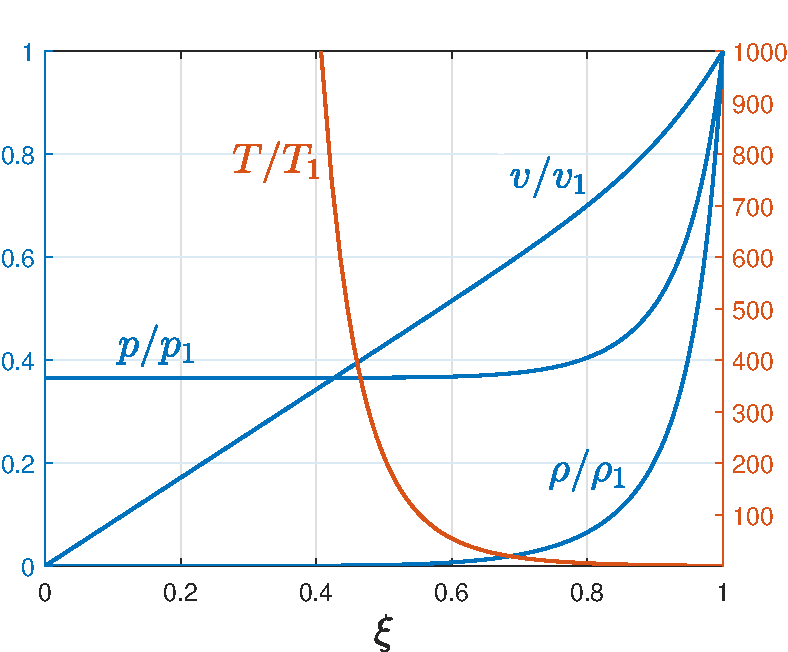
\includegraphics[height=3.5cm]{figures/TNS_blast_wave.pdf}
%            }};
%            
%        }

    \end{tikzpicture}
\end{frame}

% =============================================================================================
\section{Preliminary results}
\begin{frame}{}  %% ---------- Intro/motivation 
    \begin{tikzpicture}[overlay,remember picture]
        \uncover<1->{ % <-> |
            \node (t1) [anchor=center,scale=1,opacity=1] at ([shift={(-3.1cm,0.0cm)}]current page.center){
                \parbox{0.68\textwidth}{
                    \textbf{Emission from ``thermal" electrons}:
                    \begin{itemize}
                        \item peaks at low-$\nu$, early-$t$;
                        \item brighter for high $\Gamma\beta$, $n_0$;
                        \item evolves as ejecta decelerates;
                        \item introduces additional spectral evolution;
                        % In $\nu>1\,$GGz, emission from n is dominant ($\rho_{\rm ISM}$ is too low)
                    \end{itemize}
                    % $\{E_{\rm ej}^{\rm GRB},\Gamma_{\rm ej}^{\rm GRB}\}$,
            }};
        }
        \uncover<1-1>{ % <-> |
            \node (img1) [anchor=center,scale=1,opacity=1] at ([shift={(5.0cm,-0.3cm)}]current page.center){
                \parbox{0.5\textwidth}{
                    % \includegraphics[width=0.49\textwidth]{figs/fast_ej_fast_jet.pdf}
                    % \includegraphics[width=0.49\textwidth]{figs/slow_ej_fast_jet.pdf}
                    % \includegraphics[width=0.49\textwidth]{figs/fast_ej_slow_jet.pdf}
                    %\vspace{-5mm}
                    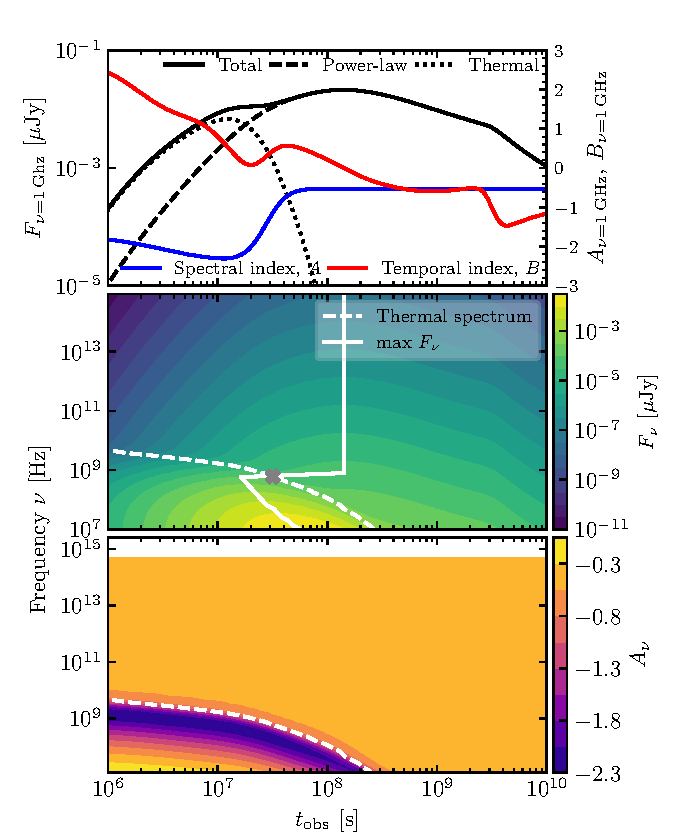
\includegraphics[width=0.45\textwidth]{../figs/fluxdens_spec_blh_q1_lk_sr.pdf}
                    %\vspace{-mm}
                    %\small{\textbf{Artist depiction of ejecta$^\text{\citep{Ascenzi:2020xqi}}$}}
            }};
        }
        %        \uncover<1-1>{ % <-> |
            %            \node (img1) [anchor=center,scale=1,opacity=1] at ([shift={(-2cm,-1.5cm)}]current page.center){
                %                \parbox{0.5\textwidth}{
                    %                    % \includegraphics[width=0.49\textwidth]{figs/fast_ej_fast_jet.pdf}
                    %                    % \includegraphics[width=0.49\textwidth]{figs/slow_ej_fast_jet.pdf}
                    %                    % \includegraphics[width=0.49\textwidth]{figs/fast_ej_slow_jet.pdf}
                    %                    %\vspace{-5mm}
                    %                    %\vspace{-mm}
                    %                    \includegraphics[width=0.48\textwidth]{../figs/comov_radio_em_pl_fast_ej_slow_jet.pdf}
                    %                    %\small{\textbf{Artist depiction of ejecta$^\text{\citep{Ascenzi:2020xqi}}$}}
                    %            }};
            %        }
    \end{tikzpicture}
\end{frame}

% =============================================================================================

\begin{frame}{}  %% ---------- Intro/motivation 
    \begin{tikzpicture}[overlay,remember picture]
        \uncover<1->{ % <-> |
            \node (t1) [anchor=center,scale=1,opacity=1] at ([shift={(-4.cm,0.6cm)}]current page.center){
                \parbox{0.54\textwidth}{
                    \textbf{Dynamics:}
                    \begin{itemize}
                        \item kilonova ejecta elements "catch-up" with GRB ejecta on various timescales; 
                        \item at "catch up" $\rho>\rho_{\rm ISM}$ and \\
                        (i) fast ones -- "break through", \\
                        (ii) slow ones -- "stall behind";%  "catching-up" %may coincide with spreading %($\Gamma^{\rm GRB}_{0}$)
                        %\item or may not occur; %($\Gamma^{\rm GRB}_{N}$)
                        \item far behind GRB ejecta, kilonova one is subsonic;
                        \item shock can form only right before the "catch up";
%                        \item 
%                        \item $\{M_{i,j}^{\rm kN}\} \gg \{M_{0}^{\rm GRB}\}$ (given layer)
%                        \item Duration of "break-through" $f(\Gamma^{\rm kN}_{\rm ej})$
%                        \item Flow largely subsonic
                    \end{itemize}
                    %\textbf{Early-time} dynamics is not significantly affected
                    %Dynamics depends on $\{E_{\rm ej}^{\rm kn},\Gamma_{\rm ej}^{\rm kn}\}$,
                    %and on the $t^{\rm GRB}_{\rm dec}$ and $c_s$. 
                    % $\{E_{\rm ej}^{\rm GRB},\Gamma_{\rm ej}^{\rm GRB}\}$,
            }};
        }
        \uncover<1-1>{ % <-> |
            \node (img1) [anchor=center,scale=1,opacity=1] at ([shift={(3.2cm,0.0cm)}]current page.center){
                \parbox{0.5\textwidth}{
                    % \includegraphics[width=0.49\textwidth]{figs/fast_ej_fast_jet.pdf}
                    % \includegraphics[width=0.49\textwidth]{figs/slow_ej_fast_jet.pdf}
                    % \includegraphics[width=0.49\textwidth]{figs/fast_ej_slow_jet.pdf}
                    %\vspace{-5mm}
                    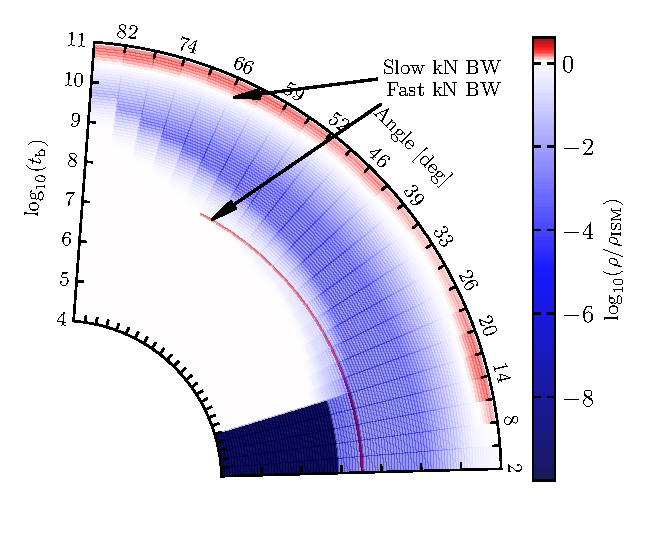
\includegraphics[width=0.60\textwidth]{../figs/dyn_ej_two_shells_angleplot.pdf}
                    %\vspace{-mm}
                    %\small{\textbf{Artist depiction of ejecta$^\text{\citep{Ascenzi:2020xqi}}$}}
            }};
        }
%        \uncover<1-1>{ % <-> |
%            \node (img1) [anchor=center,scale=1,opacity=1] at ([shift={(-2.5cm,-2.4cm)}]current page.center){
%                \parbox{0.5\textwidth}{
%                    % \includegraphics[width=0.49\textwidth]{figs/fast_ej_fast_jet.pdf}
%                    % \includegraphics[width=0.49\textwidth]{figs/slow_ej_fast_jet.pdf}
%                    % \includegraphics[width=0.49\textwidth]{figs/fast_ej_slow_jet.pdf}
%                    %\vspace{-5mm}
%                    %\vspace{-mm}
%                    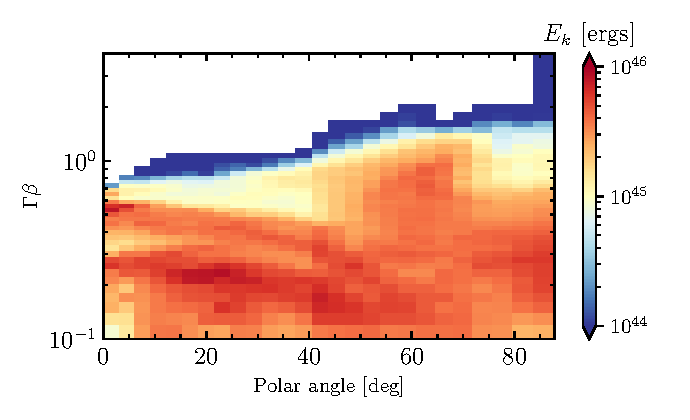
\includegraphics[width=0.40\textwidth]{../figs/ejecta_ek_dist_init_blh_q1_lk_sr.pdf}
%                    %\small{\textbf{Artist depiction of ejecta$^\text{\citep{Ascenzi:2020xqi}}$}}
%            }};
%        }
%        \uncover<1->{ % <-> |
%            \node (t1) [anchor=center,scale=1,opacity=1] at ([shift={(-3.1cm,-0.5cm)}]current page.center){
%                \parbox{0.68\textwidth}{
%                   
%            }};
%        }
        % Margalit B., Piran T., 2020, MNRAS, 495, 4981
    \end{tikzpicture}
\end{frame}



% =============================================================================================

\begin{frame}{}  %% ---------- Intro/motivation 
    \begin{tikzpicture}[overlay,remember picture]
        \uncover<1->{ % <-> |
            \node (t1) [anchor=center,scale=1,opacity=1] at ([shift={(-4.0cm,1.2cm)}]current page.center){
                \parbox{0.54\textwidth}{
                    \textbf{Change in observed radiation:}
                    \begin{itemize}
                        \item no emission from $\rho$-evacuated region;
                        \item for subsonic flow -- no shock, no emission $\rightarrow$ "Dip" in $F_{\nu}$;
                        \item at "catch-up" -- excess in $F_{\nu}$;
                        \item excess is "smeared over time" due to \\(i) kilonova ejecta structure, \\(ii) GRB lateral expansion.
                    \end{itemize}
                    %\textbf{Early-time} dynamics is not significantly affected
                    %Dynamics depends on $\{E_{\rm ej}^{\rm kn},\Gamma_{\rm ej}^{\rm kn}\}$,
                    %and on the $t^{\rm GRB}_{\rm dec}$ and $c_s$. 
                    % $\{E_{\rm ej}^{\rm GRB},\Gamma_{\rm ej}^{\rm GRB}\}$,
            }};
        }
        \uncover<1-1>{ % <-> |
            \node (img1) [anchor=center,scale=1,opacity=1] at ([shift={(3.2cm,0.0cm)}]current page.center){
                \parbox{0.5\textwidth}{
                    % \includegraphics[width=0.49\textwidth]{figs/fast_ej_fast_jet.pdf}
                    % \includegraphics[width=0.49\textwidth]{figs/slow_ej_fast_jet.pdf}
                    % \includegraphics[width=0.49\textwidth]{figs/fast_ej_slow_jet.pdf}
                    %\vspace{-5mm}
                    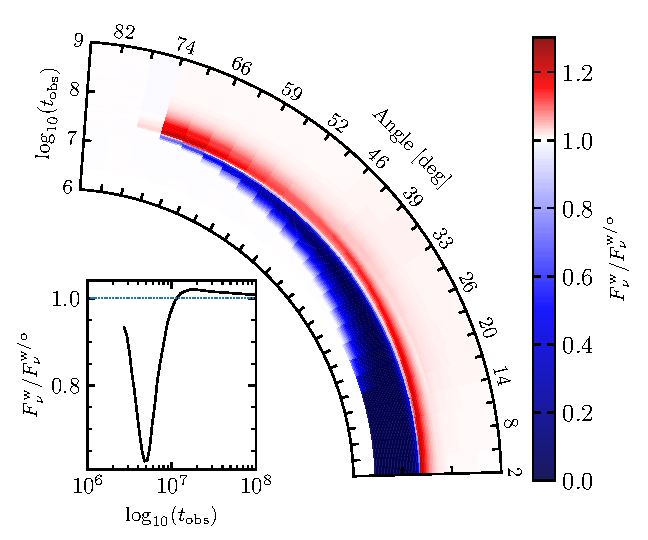
\includegraphics[width=0.60\textwidth]{../figs/lc_interaction2.pdf}
                    %\vspace{-mm}
                    %\small{\textbf{Artist depiction of ejecta$^\text{\citep{Ascenzi:2020xqi}}$}}
            }};
        }

        %        \uncover<1->{ % <-> |
            %            \node (t1) [anchor=center,scale=1,opacity=1] at ([shift={(-3.1cm,-0.5cm)}]current page.center){
                %                \parbox{0.68\textwidth}{
                    %                   
                    %            }};
            %        }
        % Margalit B., Piran T., 2020, MNRAS, 495, 4981
    \end{tikzpicture}
\end{frame}

\begin{frame}{}  %% ---------- Intro/motivation 
    \begin{tikzpicture}[overlay,remember picture]
        \uncover<1->{ % <-> |
            \node (t1) [anchor=center,scale=1,opacity=1] at ([shift={(-0.7cm,3.0cm)}]current page.center){
                \parbox{1.\textwidth}{
                    \textbf{Radio-image} $\{ \text{shape}, $\text{brightness}$ \} = f(\{E^{\rm kn}_{i, 0},\Gamma^{\rm kn}_{i,0} \})$. Dim. Require close source.
                    %                    \begin{itemize}
                        %                        \item Traces fastest ejecta geometry 
                        %                        \item Might be detectable with future observatories
                        %                    \end{itemize}
                    % $\{E_{\rm ej}^{\rm GRB},\Gamma_{\rm ej}^{\rm GRB}\}$,
            }};
        }
        \uncover<1-1>{ % <-> |
            \node (img1) [anchor=center,scale=1,opacity=1] at ([shift={(-0.5cm,-0.9cm)}]current page.center){
                \parbox{0.8\textwidth}{
                    % \includegraphics[width=0.49\textwidth]{figs/fast_ej_fast_jet.pdf}
                    % \includegraphics[width=0.49\textwidth]{figs/slow_ej_fast_jet.pdf}
                    % \includegraphics[width=0.49\textwidth]{figs/fast_ej_slow_jet.pdf}
                    %\vspace{-5mm}
                    %\vspace{-mm}
                    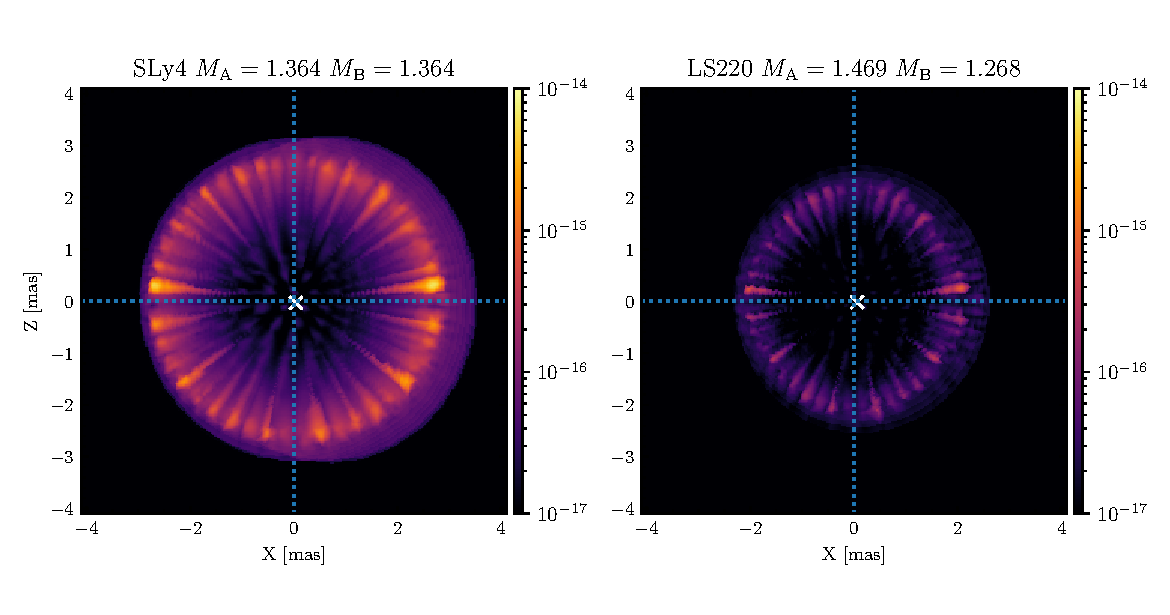
\includegraphics[width=1.\textwidth]{../figs/plot_sky_image_ejecta.pdf}
                    %\small{\textbf{Artist depiction of ejecta$^\text{\citep{Ascenzi:2020xqi}}$}}
            }};
        }
    \end{tikzpicture}
\end{frame}

%\includegraphics[width=0.49\textwidth]{figs/comov_radio_em_pl_fast_ej_slow_jet.pdf}
%\includegraphics[width=0.49\textwidth]{figs/comov_radio_em_pl_slow_ej_slow_jet.pdf}
\section{Conclusion}
\begin{frame}{}  %% ---------- Intro/motivation 
    \begin{tikzpicture}[overlay,remember picture]
        \uncover<1->{ % <-> |
            \node (t1) [anchor=center,scale=1,opacity=1] at ([shift={(-0.7cm,0.0cm)}]current page.center){
                \parbox{1.\textwidth}{
                    \textbf{Kilonova afterglow:}
                    \begin{itemize}
                        \item naturally expected if kilonova was observed;
                        \item requires close source in high density environment;
                        \item traces properties of the fastest ejecta $\rightarrow$ the mechanism of its formation;
                    \end{itemize}
                    \textbf{Thermal electron population:}
                    \begin{itemize}
                        \item dominates early- low-frequency emission;
                        \item introduces additional spectral evolution.
                    \end{itemize}
                    \textbf{Late-time kilonova- GRB- ejecta interaction:}
                    \begin{itemize}
                        \item affects early emission across all frequencies;
                        \item polar ejecta affected the most; 
                        \item interesting environment for particle acceleration.
                    \end{itemize}
            }};
        }
    \end{tikzpicture}
\end{frame}

% =============================================================================================

%\begin{frame}{}  %% ---------- Intro/motivation 
%    \begin{tikzpicture}[overlay,remember picture]
%        \uncover<1->{ % <-> |
%            \node (t1) [anchor=center,scale=1,opacity=1] at ([shift={(-0.7cm,2.5cm)}]current page.center){
%                \parbox{1.\textwidth}{
%                    \textbf{Observed emission: main features}
%                    \begin{itemize}
%                        \item Effect of jet-ISM change is minimal (but may be jet-dependent)
%                        \item If thermal electrons are considered, $F_{\rm nu}$ is much lower
%                        \item Emission is mostly from power law electrons
%                    \end{itemize}
%                    % $\{E_{\rm ej}^{\rm GRB},\Gamma_{\rm ej}^{\rm GRB}\}$,
%            }};
%        }
%        \uncover<1-1>{ % <-> |
%            \node (img1) [anchor=center,scale=1,opacity=1] at ([shift={(-2.5cm,-1.4cm)}]current page.center){
%                \parbox{0.5\textwidth}{
%                    % \includegraphics[width=0.49\textwidth]{figs/fast_ej_fast_jet.pdf}
%                    % \includegraphics[width=0.49\textwidth]{figs/slow_ej_fast_jet.pdf}
%                    % \includegraphics[width=0.49\textwidth]{figs/fast_ej_slow_jet.pdf}
%                    %\vspace{-5mm}
%                    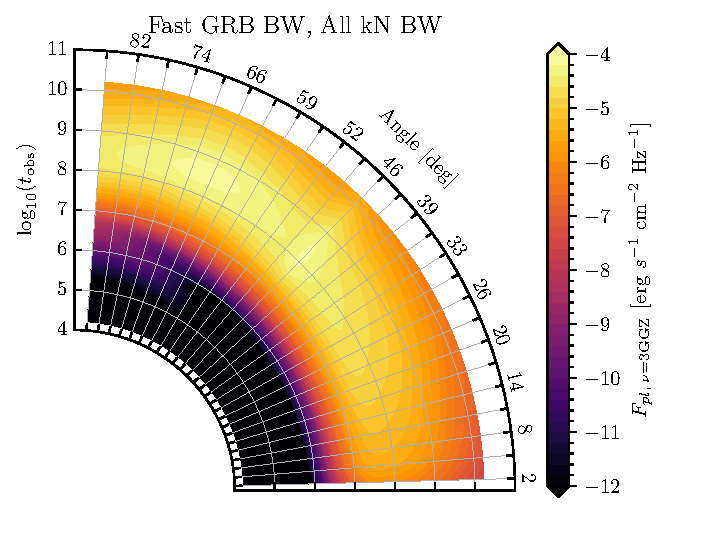
\includegraphics[width=0.50\textwidth]{../figs/observ_radio_all_ej_slow_jet.pdf}
%                    %\vspace{-mm}
%                    %\small{\textbf{Artist depiction of ejecta$^\text{\citep{Ascenzi:2020xqi}}$}}
%            }};
%        }
%        \uncover<1-1>{ % <-> |
%            \node (img1) [anchor=center,scale=1,opacity=1] at ([shift={(4.1cm,-1.5cm)}]current page.center){
%                \parbox{0.5\textwidth}{
%                    % \includegraphics[width=0.49\textwidth]{figs/fast_ej_fast_jet.pdf}
%                    % \includegraphics[width=0.49\textwidth]{figs/slow_ej_fast_jet.pdf}
%                    % \includegraphics[width=0.49\textwidth]{figs/fast_ej_slow_jet.pdf}
%                    %\vspace{-5mm}
%                    %\vspace{-mm}
%                    \includegraphics[width=0.50\textwidth]{../figs/ej_lc_jet_with_slow_jet.pdf}
%                    %\small{\textbf{Artist depiction of ejecta$^\text{\citep{Ascenzi:2020xqi}}$}}
%            }};
%        }
%    \end{tikzpicture}
%\end{frame}

% =============================================================================================



%
%% =============================================================================================
%\section{kN afterglows}
%\begin{frame}{}  %% ---------- Intro/motivation 
%    \begin{tikzpicture}[overlay,remember picture]
%        \uncover<1->{ % <-> |
%            \node (t1) [anchor=center,scale=1,opacity=1] at ([shift={(-3.1cm,-0.5cm)}]current page.center){
%                \parbox{0.68\textwidth}{
%                    \textbf{Main Features}:
%                    \begin{itemize}
%                        \item Synchrotron emission from mildly relativistic ejecta
%                        (similar to GRB afterglow and SNe remnants)
%                        %
%                        \item Expected in sGRBs but have not observed$(^*)$
%                        %
%                        \item Complex ejecta structure/geometry $\rightarrow$ non-trivial EM signature
%                        %
%                    \end{itemize}
%                    
%                    \textbf{Key Observables}: 
%                    \begin{itemize}
%                        \item $F_{\nu,p}\propto E n^{(p+1)/4}\beta^{(5p-7)/2}\varepsilon_e^{p-1}\varepsilon_B^{(p+1)/4}D_L^{-2}\nu^{(-p-1)/2}$
%                        \item $t_{p}\propto E^{1/3} n^{-1/3} \beta^{-5/3}$
%                        %
%                        \item Timescale of years.
%                        %
%                        \item Trace the properties of the fastest ejecta
%                        %
%                    \end{itemize}
%            }};
%        }
%        \uncover<1-1>{ % <-> |
%            \node (img1) [anchor=center,scale=1,opacity=1] at ([shift={(5.2cm,-4.2cm)}]current page.center){
%                \parbox{0.5\textwidth}{
%                    \includegraphics[height=8.6cm]{figures/afterglow_example.png}
%                
%                %\small{\textbf{Artist depiction of ejecta$^\text{\citep{Ascenzi:2020xqi}}$}}
%            }};
%        }
%    \end{tikzpicture}
%\end{frame}
%
%
%% =============================================================================================
%
%\section{Geometry}
%\begin{frame}{}  %% ---------- Intro/motivation 
%    \begin{tikzpicture}[overlay,remember picture]
%        \uncover<1->{ % <-> |
%            \node (t1) [anchor=center,scale=1,opacity=1] at ([shift={(-3.5cm,-0.5cm)}]current page.center){
%                \parbox{0.5\textwidth}{
%                    \textbf{Goal: combine structured GRB and kilonova afterglows}. \\
%                    \textbf{Key features}:
%                    \begin{itemize}
%                        \item lateral structure \& lateral spreading of GRB ejecta
%                        \item lateral \& velocity structure of kilonova ejecta
%                        \item GRB jet evacuates ISM in front of ejecta
%                        \item thermal electrons contribute to synchrotron emission from kilonova ejecta
%                    \end{itemize}
%            }};
%            
%        }
%        \uncover<1-1>{ % <-> |
%            \node (img1) [anchor=center,scale=1,opacity=1] at ([shift={(4.5cm,-0.3cm)}]current page.center){
%                \parbox{0.6\textwidth}{
%                    \includegraphics[height=7.8cm]{figures/structure2.pdf}
%                    %\includesvg[height=7.2cm]{figures/structure2}
%            }};
%        }
%    \end{tikzpicture}
%\end{frame}
%
%
%
%% =============================================================================================
%
%
%
%
%
%
%
%
%
%
%
%
%
%
%
%
%
%
%
%
%%\section{Phsyics}
%\subsection{Spectral evolution of GRB170817A}
%\begin{frame}{}  %% ---------- Intro/motivation 
%    \begin{tikzpicture}[overlay,remember picture]
%        \uncover<1->{ % <-> |
%            \node (t1) [anchor=center,scale=1,opacity=1] at ([shift={(-3.5cm,1.7cm)}]current page.center){
%                \parbox{0.6\textwidth}{
%                    GRB170817 from [Hajela et al 2021]:
%                    \begin{itemize}
%                        %                        \item late-time cahnge in afterglow (not a jet)
%                        \item Statistical fit indicates
%                        \textit{harder radio-to-X-ray spectrum} (lower $p$)
%                        \item Radio obs. $\rightarrow$ optically thin spectrum
%                        \item Lower $p=2$ \textit{is expected} in non-relativistic shocks (but with lower $\varepsilon_e$ as well)
%                    \end{itemize}
%                    
%            }};
%        }
%        \uncover<1-1>{ % <-> |
%            \node (img1) [anchor=center,scale=1,opacity=1] at ([shift={(5.0cm,0.1cm)}]current page.center){
%                \parbox{0.5\textwidth}{
%                    \includegraphics[height=6.5cm]{figures/figure4_2021paper.pdf}
%            }};
%        }
%        \uncover<1-1>{ % <-> |
%            \node (img1) [anchor=center,scale=1,opacity=1] at ([shift={(-3.0cm,-2.cm)}]current page.center){
%                \parbox{0.5\textwidth}{
%                    \includegraphics[height=4.5cm]{figures/SED1234days.eps}
%            }};
%        }
%    \end{tikzpicture}
%\end{frame}

